\documentclass[UTF8,a4paper,12pt]{ctexbook} 

\usepackage{graphicx}%学习插入图
\usepackage{verbatim}%学习注释多行
\usepackage{booktabs}%表格
\usepackage{geometry}%图片
\usepackage{amsmath}
\usepackage{amssymb}
\usepackage{listings}%代码
\usepackage{xcolor}  %颜色
\usepackage{enumitem}%列表格式
\setenumerate[1]{itemsep=0pt,partopsep=0pt,parsep=\parskip,topsep=5pt}
\setitemize[1]{itemsep=0pt,partopsep=0pt,parsep=\parskip,topsep=5pt}
\setdescription{itemsep=0pt,partopsep=0pt,parsep=\parskip,topsep=5pt}
\usepackage{tcolorbox}
\usepackage{algorithm}  %format of the algorithm
\usepackage{algorithmic}%format of the algorithm
\usepackage{multirow}   %multirow for format of table
\usepackage{tabularx} 	%表格排版格式控制
\usepackage{array}	%表格排版格式控制
\usepackage{hyperref} %超链接 \url{URL}

%%%% 段落首行缩进两个字 %%%%
\makeatletter
\let\@afterindentfalse\@afterindenttrue
\@afterindenttrue
\makeatother
\setlength{\parindent}{2em}  %中文缩进两个汉字位

%%%% 下面的命令重定义页面边距,使其符合中文刊物习惯 %%%%
\addtolength{\topmargin}{-54pt}
\setlength{\oddsidemargin}{0.63cm}  % 3.17cm - 1 inch
\setlength{\evensidemargin}{\oddsidemargin}
\setlength{\textwidth}{14.66cm}
\setlength{\textheight}{24.00cm}    % 24.62

%%%% 下面的命令设置行间距与段落间距 %%%%
\linespread{1.4}
\setlength{\parskip}{0.5\baselineskip}
\geometry{left=1.6cm,right=1.8cm,top=2cm,bottom=1.7cm} %设置文章宽度
\pagestyle{plain} 		  %设置页面布局

%代码效果定义
\definecolor{mygreen}{rgb}{0,0.6,0}
\definecolor{mygray}{rgb}{0.5,0.5,0.5}
\definecolor{mymauve}{rgb}{0.58,0,0.82}
\lstset{ %
	backgroundcolor=\color{white},   % choose the background color
	basicstyle=\footnotesize\ttfamily,      % size of fonts used for the code
	%stringstyle=\color{codepurple},
	%basicstyle=\footnotesize,
	%breakatwhitespace=false,         
	%breaklines=true,                 
	%captionpos=b,                    
	%keepspaces=true,                 
	%numbers=left,                    
	%numbersep=5pt,                  
	%showspaces=false,                
	%showstringspaces=false,
	%showtabs=false,        
	columns=fullflexible,
	breaklines=true,                 % automatic line breaking only at whitespace
	captionpos=b,                    % sets the caption-position to bottom
	tabsize=4,
	commentstyle=\color{mygreen},    % comment style
	escapeinside={\%*}{*)},          % if you want to add LaTeX within your code
	keywordstyle=\color{blue},       % keyword style
	stringstyle=\color{mymauve}\ttfamily,     % string literal style
	frame=single,
	rulesepcolor=\color{red!20!green!20!blue!20},
	% identifierstyle=\color{red},
	language=c++,
}
 \author{\kaishu 郑华}
 \title{Linux 系统编程 笔记}
 
\begin{document}          %正文排版开始
 	\maketitle
  
\chapter{Linux 系统编程}
	\section{虚拟地址空间}
		
	
	\section{线程}
		\subparagraph{pthread\_create}

		\verb|pthread_create(pthread_t*  id, pthread_attr_t* attr, void*(*start_routine)(void*), void* arg)|
		
		\begin{itemize}
			\item \verb|void* (*start_routine) (void*)|:这里是个陷阱,如果使用成员函数会存在一个参数不匹配问题,因为成员函数有一个隐含的第一参数this,而this 为类指针类型,与void* 不匹配,造成了notMatch 错误。
		\end{itemize}
				 
	\section{进程}
		\subsection{进程空间}
			\url{http://www.cnblogs.com/xzzzh/p/6596982.html}
			
			\url{http://www.cnblogs.com/smile267/archive/2012/10/21/2732099.html}
		\subsection{uid、euid}
		
		\subsection{fork}
			fork之后子进程到底复制了父进程什么? \url{http://blog.csdn.net/xy010902100449/article/details/44851453}
			
			
			这里就涉及到物理地址和逻辑地址(或称虚拟地址)的概念。
			
			从逻辑地址到物理地址的映射称为地址重定向。分为:
			
			静态重定向--在程序装入主存时已经完成了逻辑地址到物理地址和变换,在程序执行期间不会再发生改变。
			
			动态重定向--程序执行期间完成,其实现依赖于硬件地址变换机构,如基址寄存器。
			
			逻辑地址:CPU所生成的地址。CPU产生的逻辑地址被分为 :p (页号) 它包含每个页在物理内存中的基址,用来作为页表的索引;d (页偏移),同基址相结合,用来确定送入内存设备的物理内存地址。
			
			物理地址:内存单元所看到的地址。
			用户程序看不见真正的物理地址。用户只生成逻辑地址,且认为进程的地址空间为0到max。物理地址范围从R+0到R+max,R为基地址,地址映射-将程序地址空间中使用的逻辑地址变换成内存中的物理地址的过程。由内存管理单元(MMU)来完成。
			
			fork()会产生一个和父进程完全相同的子进程,但子进程在此后多会exec系统调用,出于效率考虑,linux中引入了“写时复制“技术,也就是只有进程空间的各段的内容要发生变化时,才会将父进程的内容复制一份给子进程。在fork之后exec之前两个进程用的是相同的物理空间(内存区),子进程的代码段、数据段、堆栈都是指向父进程的物理空间,也就是说,\textbf{两者的虚拟空间不同,但其对应的物理空间是同一个}。\textbf{当父子进程中有更改相应段的行为发生时,再为子进程相应的段分配物理空间},如果不是因为exec,内核会给子进程的数据段、堆栈段分配相应的物理空间(至此两者有各自的进程空间,互不影响),\textbf{而代码段继续共享父进程的物理空间}(两者的代码完全相同)。而如果是因为exec,由于两者执行的代码不同,子进程的代码段也会分配单独的物理空间。
			
			\textbf{fork时子进程获得父进程数据空间、堆和栈的复制,所以变量的地址(当然是虚拟地址(相对位置))也是一样的}。
			
			\textbf{每个进程都有自己的虚拟地址空间},不同进程的相同的虚拟地址显然可以对应不同的物理地址。因此地址相同(虚拟地址)而值不同没什么奇怪。
			具体过程是这样的:
			fork子进程完全复制父进程的栈空间,也复制了页表,但没有复制物理页面,所以这时虚拟地址相同,物理地址也相同,但是会把父子共享的页面标记为“只读”(类似mmap的private的方式),如果父子进程一直对这个页面是同一个页面,知道其中任何一个进程要对共享的页面“写操作”,这时内核会复制一个物理页面给这个进程使用,同时修改页表。而把原来的只读页面标记为“可写”,留给另外一个进程使用。
			
			这就是所谓的“写时复制”。正因为fork采用了这种写时复制的机制,所以fork出来子进程之后,父子进程哪个先调度呢?内核一般会先调度子进程,因为很多情况下子进程是要马上执行exec,会清空栈、堆。。这些和父进程共享的空间,加载新的代码段。。。,这就避免了“写时复制”拷贝共享页面的机会。如果父进程先调度很可能写共享页面,会产生“写时复制”的无用功。所以,一般是子进程先调度滴。
			
			\textbf{假定父进程malloc的指针指向0x12345678, fork 后,子进程中的指针也是指向0x12345678,但是这两个地址都是虚拟内存地址 (virtual memory),经过内存地址转换后所对应的 物理地址是不一样的。所以两个进程中的这两个地址相互之间没有任何关系。}
			
			
			(注1:在理解时,你可以认为fork后,这两个相同的虚拟地址指向的是不同的物理地址,这样方便理解父子进程之间的独立性)
			(注2:但实际上,Linux为了提高 fork 的效率,采用了 copy-on-write 技术,fork后,这两个虚拟地址实际上指向相同的物理地址(内存页),只有任何一个进程试图修改这个虚拟地址里的内容前,两个虚拟地址才会指向不同的物理地址(新的物理地址的内容从原物理地址中复制得到))
	\section{共享内存区}
	
	\section{消息队列}
	
	\section{信号量}
	
	\section{库的使用}
		\url{http://www.cnblogs.com/52php/p/5681711.html}
		\subsection{介绍}
			使用GNU的工具我们如何在Linux下创建自己的程序函数库?一个“程序函数库”简单的说就是一个文件包含了一些编译好的代码和数据,这些编译好的代码和数据可以在事后供其他的程序使用。程序函数库可以使整个程序更加模块化,更容易重新编译,而且更方便升级。  
			
			引用的那些\textbf{头文件中的函数}是怎么被执行的呢?这就要牵扯到\textbf{链接库}了!
			
			库有两种,一种是 \textbf{静态链接库},一种是 \textbf{动态链接库},不管是哪一种库,\textit{要使用它们,都要在程序中包含相应的 include 头文件}。编译过程如下:
			
			\begin{figure}[h]
				\centering
				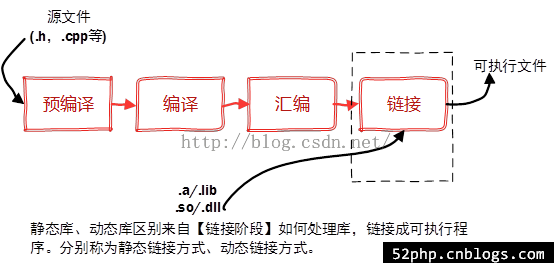
\includegraphics[scale = 0.7]{figure/compileProcess.png}
				\caption{编译过程}
			\end{figure}
			
			\verb|gcc -o helloWorld helloWorld.c| 生成一个helloWorld 的执行文件,格式为ELF(与widows的exe类似)。
			
		\subsection{静态函数库}是在程序执行前就加入到目标程序中去了;
		
			静态函数库实际上就是简单的一个普通的目标文件的集合,一般来说习惯用“\verb|.a|”作为文件的\textbf{后缀}
			
			静态库函数允许程序员把程序link起来而不用重新编译代码,节省了重新编译代码的时间。
			
			如你想把自己提供的函数给别人使用,但是又想对函数的源代码进行保密,你就可以给别人提供一个静态函数库文件。理论上说,使用ELF格式的静态库函数生成的代码可以比使用共享函数库(或者动态函数库)的程序\textbf{运行速度上快一些,大概1-5\%,但是占用空间却大了很多。}
			
			\subparagraph{Example}\verb|->|
				
				定义一个加法函数,做成静态库,首先需要将声明放到头文件以便引用。
				\begin{lstlisting}
	// add.h
	#ifndef _ADD_
	#define _ADD_
	#include <iostream>
	
	int add(int a, int b);
	#endif
				\end{lstlisting}
				
				实现该函数
				\begin{lstlisting}
	#include "add.h"
	
	int add(int a, int b)
	{
		return a+b;
	}
				\end{lstlisting}
			
				生成静态库:
				\begin{enumerate}[itemindent = 2em]
					\item \verb|g++ -c add.cc|生成\verb|.o|文件
					\item \verb|ar -crv libadd.a add.o|生成一个静态库
				\end{enumerate}
				
				
				测试:
				\begin{lstlisting}
	//目录结构
	project
		|
		+---Main.cc
		|
		+---addlib
				|
				+----add.h
				|
				+----add.cc
	
	#include <iostream>
	#include "./addlib/add.h"
	
	using namespace std;
	int main()
	{
		int num1 = 10;
		int num2 = 90;
		cout <<"the result is"<< add(num1,num2)<<endl;
		return 0;
	}
				\end{lstlisting}
				不管是哪一种库,\textit{要使用它们,都要在程序中包含相应的 include 头文件},所以include使用相对路径找到头文件\verb|add.h|
				
				然后我们使用\verb|g++ -o Test Main.cc -L ./addlib/ -ladd| 进行编译
				
				\begin{itemize}[itemindent = 2em]
					\item \verb|L |是指定加载库文件的路径
					\item \verb|l |是指定加载的库文件
				\end{itemize}
				
			\subparagraph{静态库搜索路径}\verb|->|
			
				\begin{enumerate}[itemindent= 2em]
					\item 编译目标代码时指定的静态库搜索路径。 \verb|-L ./src/ -lpthread|
					\item 环境变量\verb|LIBRARY_PATH| 指定的动态库搜索路径。
					
					 \verb|   export LIBRARY_PATH=/opt/lib:$LIBRARY_PATH|
					\item 配置文件\verb|/etc/ld.so.conf| 中指定的动态库搜索路径,然后运行\verb|/sbin/ldconfig|刷新缓存
					\item 默认的动态库搜索路径\verb|/lib, /usr/lib|
				\end{enumerate}
				
		\subsection{动态函数库}
			静态链接的话,文件会很大,往往实现很小的一个功能就需要占用很大的空间,而且每次库文件升级的话,都要重新编译源文件,很不方便。如下:
			\begin{figure}[h]
				\centering
				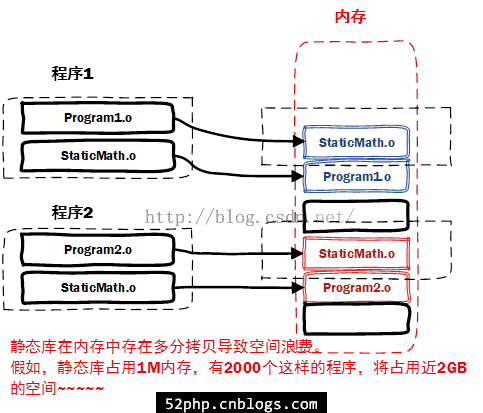
\includegraphics[scale = 0.7]{figure/staticLib-disAdvantage.png}
				\caption{静态库冗余空间}
			\end{figure}
			
			对于静态编译的程序1和程序2,都应用库staticMath。在内存中就又\textbf{两份相同的staticMath目标文件,很浪费空间},一旦程序数量过多就很可能会内存不足。
			
			这么大的内存才只能运行这几个程序,实在不甘心。
			这样就又了动态库发挥威力的地方了。我们来看看动态链接的结果:
			
			\begin{figure}[h]
				\centering
				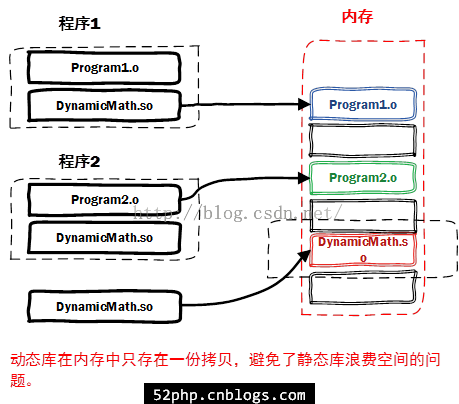
\includegraphics[scale = 0.7]{figure/dynamicLib.png}
				\caption{动态库解决静态库冗余空间问题}
			\end{figure}

			在这种模型中,两个程序只应用一个库,这个目标文件在内存中只有一份,供所有程序使用。
			并且在程序运行过程中动态调用库文件,\textbf{很方便,又不占空间},但是动态链接有一个\textbf{缺点就是可移植性太差},如果两台电脑运行环境不同,动态库存放的位置不一样,很可能导致程序运行失败。
			
			\subparagraph{Example}使用静态库代码结构与代码
			
			生成一个\verb|libadd.so|的动态库
			\verb|g++ -fPIC -shared -o libadd.so add.cpp|。
			这样就生成一个了一个libadd.so 的动态库。
			
			
			使用如下命令进行编译:
			\verb|g++ -o Test Main.cc -L ./addlib/ -ladd -Wl,-rpath=./addlib/|
			
			但是如果不指定运行时搜索路径的话,会出现cannot open shared obj错误。如下编译:
			
			\verb|g++ g++ -o Test Main.cc -L ./addlib/ -ladd|
			
			此时可以通过\verb|ldd ./Test|进行查看调用的动态库情况。具体的设置可参考动态库搜索路径的4种方法。
			
			
			\subparagraph{动态库搜索路径}\verb|->|
			
				\url{http://blog.csdn.net/weicao1990/article/details/51028335}			
				\url{https://www.cnblogs.com/cute/archive/2011/02/24/1963957.html}
				
				\begin{enumerate}[itemindent= 2em]
					\item 编译目标代码时指定的动态库搜索路径。\verb|-L./src/ -ladd -Wl,-rpath=./src/|
					
					\verb|   |前面两个\verb|-L -l|分别指明了动态库的位置和库的名字用于编译,只有引用, 后面的\verb|-Wl,-rpath|则指明运行时到哪里运行,有内容。
					
					\item 环境变量\verb|LD_LIBRARY_PATH| 指定的动态库搜索路径。
					
					\verb|   export LD_LIBRARY_PATH=/opt/lib:$LD_LIBRARY_PATH|
					\item 配置文件\verb|/etc/ld.so.conf| 中指定的动态库搜索路径,然后运行\verb|/sbin/ldconfig|刷新缓存
					\item 默认的动态库搜索路径\verb|/lib, /usr/lib|,\verb|mv ./src/xx.lib  /lib|
				\end{enumerate}
				    
\end{document} 
 		    